\documentclass[amsmath,amssymb,reprint,
tightenlines,aps,prl,11pt]{revtex4-1}

\usepackage{fancyhdr}
\pagestyle{fancy}
\lhead{Monte Carlo Simulations of Galaxy Formation and Evolution}
\rhead{u5561093}

\usepackage{graphicx,placeins}% Include figure files
\usepackage{graphicx}
\usepackage{eqnarray}

%% This assignment
\usepackage[margin=0.8in]{geometry}
\usepackage{adjustbox}
\graphicspath{{code/}}
\usepackage{subcaption,caption,placeins}
\usepackage{color}
\usepackage{listings}
\lstset{
    frame       = single,
    numbers     = left,
    showspaces  = false,
    showstringspaces    = false,
    captionpos  = t,
    caption     = \lstname,
    breaklines 	=true,
 	postbreak 	=\mbox{\textcolor{red}{$\hookrightarrow$}\space},
}


\bibliographystyle{ieeetran}

\begin{document}

\title[PHYS3103 Essay]{Monte Carlo Simulations of Galaxy Formation and Evolution}% Force line breaks with \\

\author{Uri Pierre Burmester (u5561093) - Australian National University}%Lines break automatically or can be forced with \\

\date{\today}

\begin{abstract}
This paper is an overview of the applications of Monte Carlo Methods (MCMs) to studying galaxy formation and evolution. An introduction to the astrophysics underlying the current theories of galaxy formation is given, including the Lambda Cold Dark Matter model and some background into the types and properties of galaxies. Next, the paper covers the basic premises of a Monte Carlo analysis. Then several papers are discussed as representatives of  the current body of work, including strengths and weaknesses of the approaches. Lastly, simulation results are shown illustrating how MCMs can be used to estimate the fractal dimension of spiral galaxies, based on the work of Yoshino and Sagawa \cite{yoshinoMONTECARLOSIMULATION2008}.
\end{abstract}

\maketitle

\section{Introduction \label{sec:introduction}}

In the past two decades, scientific papers on the topic of galaxy formation and evolution have exploded in popularity. This interest owes partly to the continual improvement of astronomical equipment such as the construction of ever-larger telescopes and more precise optics, allowing for observations of fainter and more distant objects. However, another contributing factor is the dramatic increase in the availability, speed and usability of computing power. While semi-analytical models purporting to describe galactic processes have existed for some time \cite{silkCosmicBlackBodyRadiation1968, peeblesBlackBodyRadiationContent1965}, these do not have closed-form solutions nor easily-measurable parameters, making numerical methods a vital tool for evaluating our models and comparing them with observations. This paper introduces some of the physical models underlying galaxy formation and evolution, introduces Monte Carlo Methods (MCMs) which can be applied to these situations and discusses the benefits and limitations of these approaches. Lastly, a simplified model of galaxy formation from Yoshino and Sagawa is replicated to demonstrate the principle \cite{yoshinoMONTECARLOSIMULATION2008}.

\section{Properties of galaxies}
The central question of galaxy formation can be understood by considering the state of the universe at the present time and comparing it to a time shortly after the Big Bang. The early universe was extremely hot and very homogeneous, containing only hydrogen and helium. In the present day, however, the universe is very inhomogenous on large length scales - intergalactic space has a density of only around one atom per cubic metre, with distances between galaxies in the millions of light-years \cite{BigBangModel2019}. Inside galaxies however, hundreds of billions of stars are crowded into a space only thousands of light-years across. This transition from a homogeneous to an inhomogeneous universe is what models of galaxy formation and evolution seek to explain \cite{FormationGalaxies2019}. \\

Models of galaxy formation and evolution need to accurately predict more than simply the existence and mass of galaxies, though. Galaxies have several other distinguishing properties which these models seek to fit. One of these is morphology, or galaxy shape; galaxies can be broadly grouped into elliptical, spiral and spiral barred based on their shape. Spiral galaxies also belong to the class of 'disk galaxies'. Galactic discs consist of a stellar component (composed of most of the galaxy's stars) and a gaseous component (mostly composed of cool gas and dust)  \cite{FormationGalaxies2019}. Some of the more common galaxy morphologies are shown in Hubble's classification system, as shown in Figure \ref{fig:tuning-fork}. Other properties include metallicity (the proportion of observable mass made up of atoms heavier than hydrogen and helium) and fractal dimension, $D$. This last measure is important to determine as the large-scale structure of matter in the universe is often modelled as a scale-invariant fractal of dimension $D$. \\

\begin{figure} \centering
\includegraphics[width=0.7\columnwidth]{tuning-fork.jpg}
\caption{Galaxy Morphology Classification System proposed by Edwin Hubble. Source: \cite{HubbleTuningFork}}
\label{fig:tuning-fork}
\end{figure}

These explanations must also take into account a model of dark matter, which is hypothesised to make up the majority of mass in galaxies despite not interacting via the electromagnetic force. Measurements of the rotations of galaxies' outer stars reveal that these stars rotate faster than would be possible for a galaxy containing only baryonic matter. Dark Matter 'halos' are hypothesised to envelop the galactic disc and extend well beyond the edge of the visible galaxy \cite{GalaxyEvolutionGalaxies}.

\section{Existing Models}
'Bottom-up' models of galaxy formation have been gaining increasing acceptance among astrophysicists. The Lambda Cold Dark Matter (LCDM) model is one such model which posits that the universe contains cold dark matter (CDM). The "cold" in this case refers to the average speed of the dark matter particles, they are relatively slow compared to the speed of light \cite{FormationGalaxies2019}. Slight differences in the density of the primordial universe during its inflationary stage can be observed in the cosmic microwave background radiation. These mass overdensities attract more mass than less dense areas, causing the disparity in density to grow and allowing galaxies to accumulate mass by clustering and merging. The Press-Schechter formalism is one of the most widely used mathematical formalisms for understanding this - it attempts to predict the number of objects (e.g. galaxies, galaxy clusters, dark matter halos) of given mass within a universe of given cosmological properties \cite{pressFormationGalaxiesClusters1974}. Press and Schechter predict that in a scale-free power spectrum, the number of objects between masses $M$ and $M+dM$ is $dn$.

\begin{equation}
M \frac{d n}{d M}=\frac{1}{\sqrt{\pi}} \frac{\overline{\rho}}{M}\left(\frac{M}{M^{*}}\right)^{1 / 2} e^{-M / M^{*}}
\end{equation} 

Where $M^{*}$ is a cut-off mass below which structures will form and $\bar{\rho}$ is the mean (baryonic and dark) matter density of the universe during the period of the initial mass fluctuation. The Press-Schechter formalism is derived by assuming that each object is formed by gravitational collapse of a density fluctuation. \cite{pressFormationGalaxiesClusters1974}. 

\section{Monte Carlo Methods} 

In many ways, galactic evolution is very well suited to numerical simulation. The dynamics are very easily expressible in terms of individual stars, which are a useful discrete 'particle' on which to base a simulation. The relative emptiness of the universe also makes the physical situations simple to model because of the absence of most disperse forces such as friction and air resistance. The relative abundance of stars in the observable universe and long timescales of astronomical systems also assures that stars as a whole can be well-approximated by statistical distributions \cite{paltaniMonteCarloMethods2011}. \\

Monte Carlo Methods are one such set of computational tools. Fundamentally, the principle underlying these algorithms is repeated random sampling. By utilising many random samplings, we are able to simulate an effect which may be deterministic in principle. The three most common applications of this are: numerical integration, optimisation and generating draws from a random distribution. N-Body Monte Carlo simulations can be used for all three of these applications; the classic example of this is using $N$ randomly distributed particles in a square of area $A$ to estimate the value of $\pi$. As $n \rightarrow \infty$, $\pi$ can be approximated as

\[ \pi = \lim_{n \rightarrow \infty} 4 \frac{N_c}{N} \]

where $N_c$ is the number of particles inscribed in the circle. An example of the third application is the so-called Markov-Chain Monte Carlo (MCMC) method. When a random distribution is known, a Markov chain model can be designed that will approximate this probability distribution in the limit as the number of steps goes to infinity. One application of this is calculating the conditional probability $P(D|x)$ that a given data set $D$ occurs given the values of some model parameters, $x$. Bayes' Theorem states that, given a prior $P(x)$, the posterior probability of the model $\pi(x)$ is 

\[ \pi(x) \propto P(D|x) P(x) \]

\cite{paltaniMonteCarloMethods2011}. A MCMC method then simply steps from one point in the sample space to the next, choosing from a distribution that depends only on the preceding point. This can be thought of like traversing a tree where nodes are connected by edges with associated probabilities. The main advantage of MCMC is that the posterior distribution and correlations for the parameters can be recovered from the sample list and the un-normalised probability \cite{paltaniMonteCarloMethods2011}.

\section{MCM for simulating galactic evolution and formation}

Knowing this background, we can see some examples of MCMs in use in astrophysics. One application is simulating the type and distribution of isotopes present in a galaxy during its lifetime. This is a 'Galactic Chemical Evolution' model and aims to provide an estimate of the Star Formation Rate (SFR), initial mass function (IMF), types and occurrences of supernovae (SN Ia, Ib/c, II) and the stellar nucleosynthetic contributions of stars with distinct mass and metallicity. Sahjipal and Kaur instead approached this problem using an N-Body Monte Carlo simulation, where each 'particle' was a star with a mass between 0.1 to 100 solar masses. Stars were tracked inside a simulated galaxy that was divided into annular rings using a stellar number distribution function $G_i(t, m)$, where $G_i$ gave the number of stars of a particular mass $m$ at time $t$ in ring $i$. Sahjipal and Kaur adopted a two/three infall accretion model, where galaxy halo was formed first and the galactic halo was formed second from the gradual accumulation of intergalactic gas \cite{sahijpalMonteCarloBased2018}. 

The simulation timestep was $10^6$ years. Each of the annular rings evolved distinctly in terms of star formation and stellar nucleosynthesis, with some mixing of interstellar gas taking place between the rings in each timestep. After each timestep, new stars are formed based on the availability of gas in each ring, the star formation rate, and metallicity. The stellar ejecta from these stars are homogenized instantaneously within the entire annular ring, thereby enriching the metallicity of the ring. The nucleosynthetic yields of the stars were based on stellar surveys \cite{sahijpalMonteCarloBased2018}. 

After completing thousands of simulations including various different initial conditions, Sahijpal and Kaur concluded that the Milky Way accreted during the initial stages ($\leq 1 Gyr$) to form the halo, then later the disc. They also concluded that the  three-infall accretional model seems to be the most viable scenario that explains the majority of the evolutionary features related to the elemental abundance distributions and gradients. Using an N-body simulation in this case provided significant advantages over past methods in order to reach these conclusions. Previous models, such as those based on Press-Schechter theory, relied on a complex set of differential equations which were based on (possibly incorrect) assumptions about the formation and evolution of the galacic halo and disc \cite{sahijpalMonteCarloBased2018}. The MCM simulation also better accounts for the radial flow of isotopes than do differential equation models. Astronomical observations indicate that stars drift away from their birthplaces, influencing the chemical and kinematical properties of the galactic disc. Intragalactic gas is also observed to experience radial flow, influencing chemical abundance within galaxies \cite{sahijpalMonteCarloBased2018}. 

There are also drawbacks to this model, though. In simplifying the underlying dynamics, the MCM risks losing important features of the system. For example, Sahjipal and Kaur's simulation assumes the stellar ejecta at each timestep are immediately mixed across the whole annular ring, an assumption that certainly wouldn't be true of a spiral galaxy which has alternating bands of high and low stellar density. The timestep of $10^6$ years is also necessary for computational expediency and would represent the lifespan of most stars well; however, very large stars have lifespans on the order of $10^6$ years, meaning their dynamics are practically not modelled at all. Choosing a timestep, scale and update equations to balance computational complexity and the complexity of the underlying system is a perennial problem of these kinds of simulations. \\

Henriques et al. are a good example of using MCMC methods to model galaxy formation. They used the data created by the Millennium dark matter simulation to explore the relevant cosmological parameter space. This simulation used the evolution of more than 10 billion particles in a simulated universe over 2 billion light-years on a side, creating terabytes of data. Scientists such as  Springel et al. then coupled these large datasets to Semi-Analytic (SA) models in an attempt to create models of interstellar dust, galaxy mergers and other phenomena \cite{springelSimulatingJointEvolution2005}. These models could be made to reproduce many observable properties however Henriques et al. observed that the choice of parameters used for these models had never been studied in a statistically consistent way. Some of these properties include the cosmic baryon fraction, star formation frequency, hot gas black hole accretion rate, etc. The large number of observational properties that galaxy formation models attempt to predict requires a large number of parameters (some of which are strongly correlated). This causes considerable difficulties in determining how to improve the agreement with new observations without destroying the match with existing data sets \cite{henriquesMonteCarloMarkov2009}. 

These difficulties can be overcome by combining multiple observations with proper sampling of high-dimensional parameter spaces, which Henrique et al. accomplish by applying MCMC methods to the semi-analytic (SA) model created by Springel et al. \cite{springelSimulatingJointEvolution2005}. Henrique et al. sampled a subset of the Millennium dataset at each MCMC step, running the SA model with the proposed set of parameters and computing the acceptance probability by comparing the outputted galaxy properties with the observational constraints \cite{henriquesMonteCarloMarkov2009}. One of these was by comparing the model with obsevations of the K-Band (infrared) luminosity distribution using a $\chi^2$ probability test. The researchers then produced one- and two-dimensional maximum likelihood  and MCMC posterior distributions, allowing them to quantify the correlation between the sets of simulation parameters. They then repeated this analysis using other features to obtain mean values, confidence limits and likelihood contours for the best-fitting models. Ultimately, Henrique et al. find that the previously published parameter values lie within their confidence limits \cite{henriquesMonteCarloMarkov2009}. 

One of the main advantages of this work is that it provides a statistically rigorous way of demonstrating the correlation between sets of simulation parameters, which provides a strong indication of an underlying deterministic relationship between those variables. Additionally, by placing confidence intervals on the best-fit parameters, researchers are able to make informed choices about which simulation values are well known versus those that have a high uncertainty. One disadvantage of using these statistical tests to form a confidence interval is that the results are only as reliable as observational datasets against which they are compared. If they contain some systematic error, for example, this will propagate into the prior/posterior distributions and taint the results. 

\section{Simulating Result from Yoshino and Sagawa}

Yoshino and Sagawa are primarily interested in exploring the homogeneity of the universe at different length scales, as this is vital to understanding the process of galaxy formation. This paper is primarily focused on spiral galaxies and quantifies the homogeneity using the fractional dimension. Historically, the fractal dimension of the large scale matter distribution in the universe was first
discussed by Peebles \cite{peeblesBlackBodyRadiationContent1965}, who predicted a value of $D = 1.2$ in a universe whose scale is smaller than 20 MPc. Elmegreen obtained the fractal dimensions from the observations of several star formations in the spiral
galaxy NGC 2207; he found a value $D = (1.12 \pm 0.25)$ \cite{peeblesBlackBodyRadiationContent1965}. Thanki also analyzed the intensity levels of spiral galaxy images and showed that the fractal dimensions spread from 0.8 to 1.5 with the average around 1.2. Yoshino and Sagawa attempt to construct a stochastic model which results in the same behaviour \cite{yoshinoMONTECARLOSIMULATION2008}. The next paragraphs describe Yoshino and Sagawa's methodology, which was also used in our replication simulation.

We require a model of stellar evolution. Large stars typically live for around $10^6$ years before undergoing a series of rapid expansions and contractions which lead to an explosive supernova. The force of this explosion propels the gasses which made up the star hundreds of parsecs, forming new clouds with different areas of inhomogeneous density. This leads to the formation of new stars. 

Our model consists of a polar grid of $Nr = 149$ concentric rings, each with $6N$ cells (where $N$ is the ring number). These cells are 100pc in size, corresponding to a typical galactic radius of 150 kpc. Assume a rotation of the cells of $Vr = 2 cells/\Delta t$ ($200 km/s$), for a time step of $\Delta t = 10^6 yrs$. Lastly, we randomly populate 2 \% of the cells in the inner 120 rings with large stars with a lifespan of $10^6 yrs$. Every timestep, these stars experience a supernova and their shockwave is transmitted to the adjacent cells at a speed of $V_{sw} = 0.2 cells/ \Delta t$, as shown in Figure \ref{fig:setup}. Each of these 'neighbour' cells will form a new star with a probability $P_{sw} = 0.183$.  \\

\begin{figure}
\centering
\begin{adjustbox}{center}
\includegraphics[width=0.7\columnwidth]{polarGrid.png}
\end{adjustbox}
\caption{Polar array used to simulate galaxy formation. Source: \cite{yoshinoMONTECARLOSIMULATION2008}}
\label{fig:setup}
\end{figure}

Our replication of these results is shown in Figure \ref{fig:beforeAfter}. It is clear that this method visually achieves some success in modelling the formation of spiral galaxies. The authors were able to achieve convincing spiral galaxy shapes after only 100 timesteps (i.e $100 Myr$) after which the shape remained stable; this was consistent with our results. The probabilistic element of the simulation lies in the random initial distribution of the large stars and in the probabilistic method of star formation. This allows us to make an empirical argument about the role played by supernovae in the formation of the spiral galaxy structure without constructing an unwieldy analytical model. The fractal dimension is then computed using a two-point correlation method, which gives an estimated fractal dimension of $D = 1.25$ \cite{yoshinoMONTECARLOSIMULATION2008}. This experiment was then repeated using a more complicated stochastic model with different star types and different gas densities across the array, but the result was similar.

\begin{figure}[]
        \centering
        \begin{subfigure}[]{0.9\columnwidth}
            \centering
            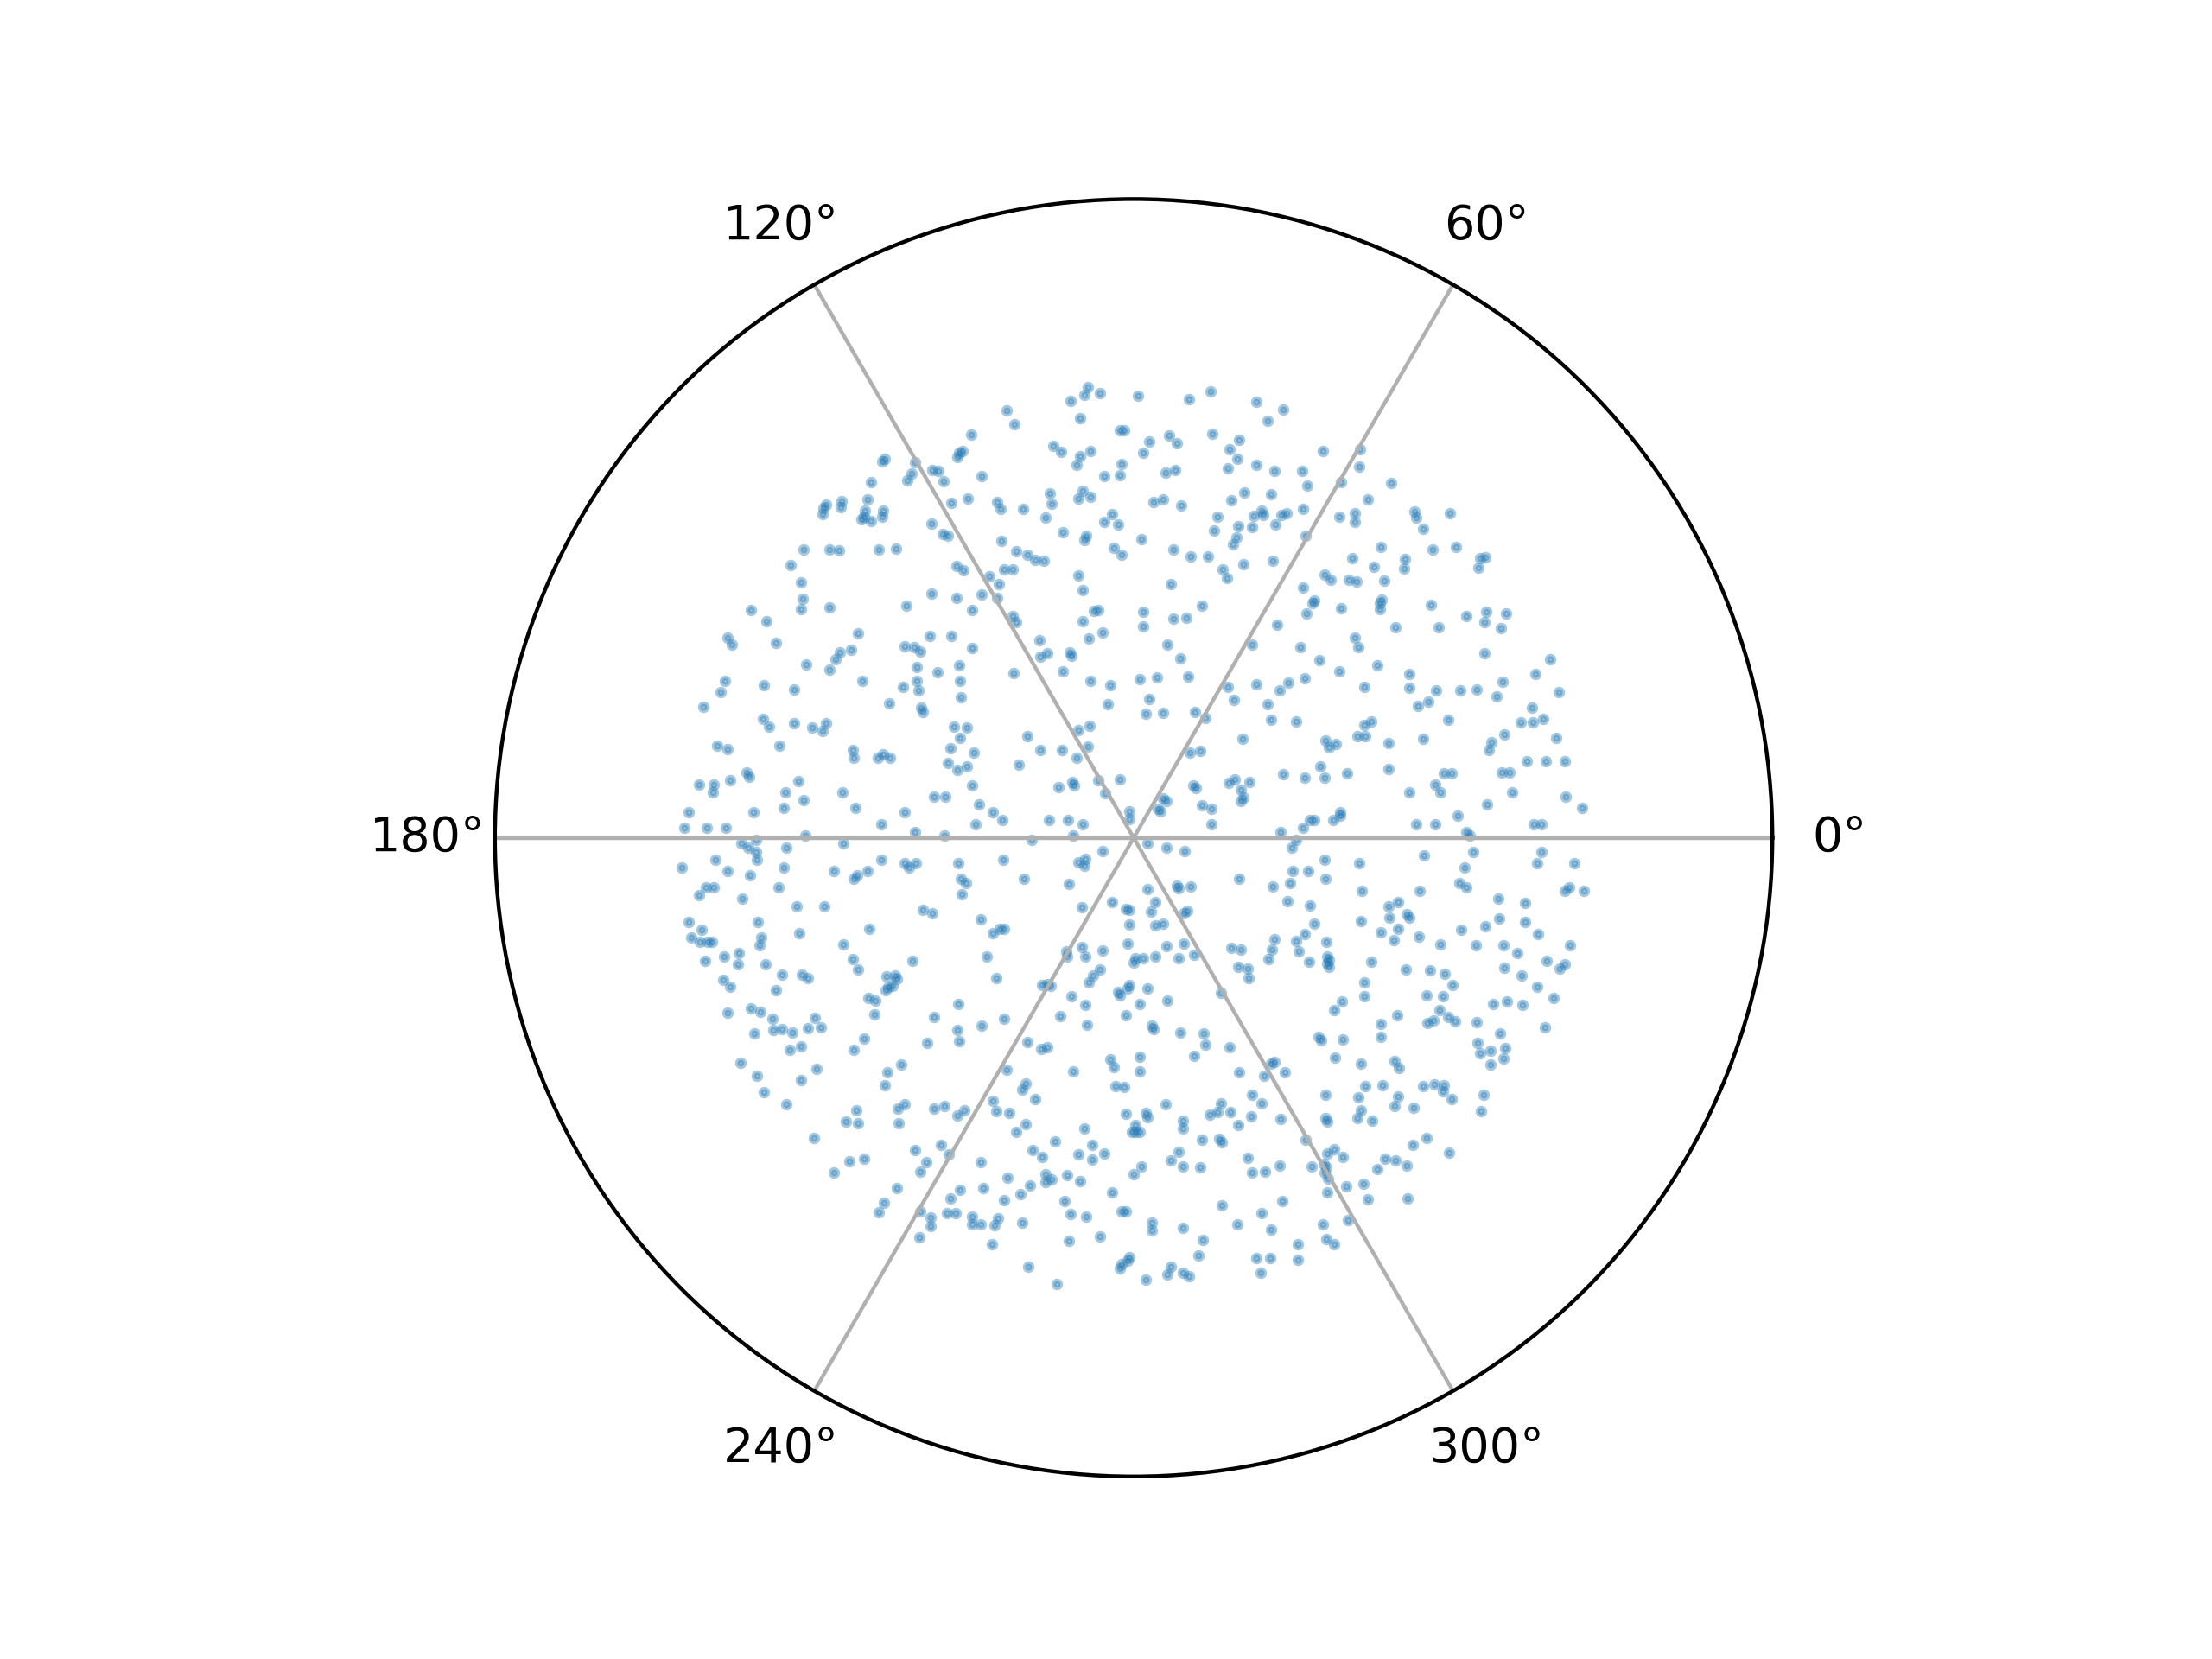
\includegraphics[width=\columnwidth]{galaxySimulationBefore.png}
            \caption{Initial, random star distribution}
            \label{fig:before}
        \end{subfigure}
        \hfill
        \begin{subfigure}[]{\columnwidth}
            \centering
            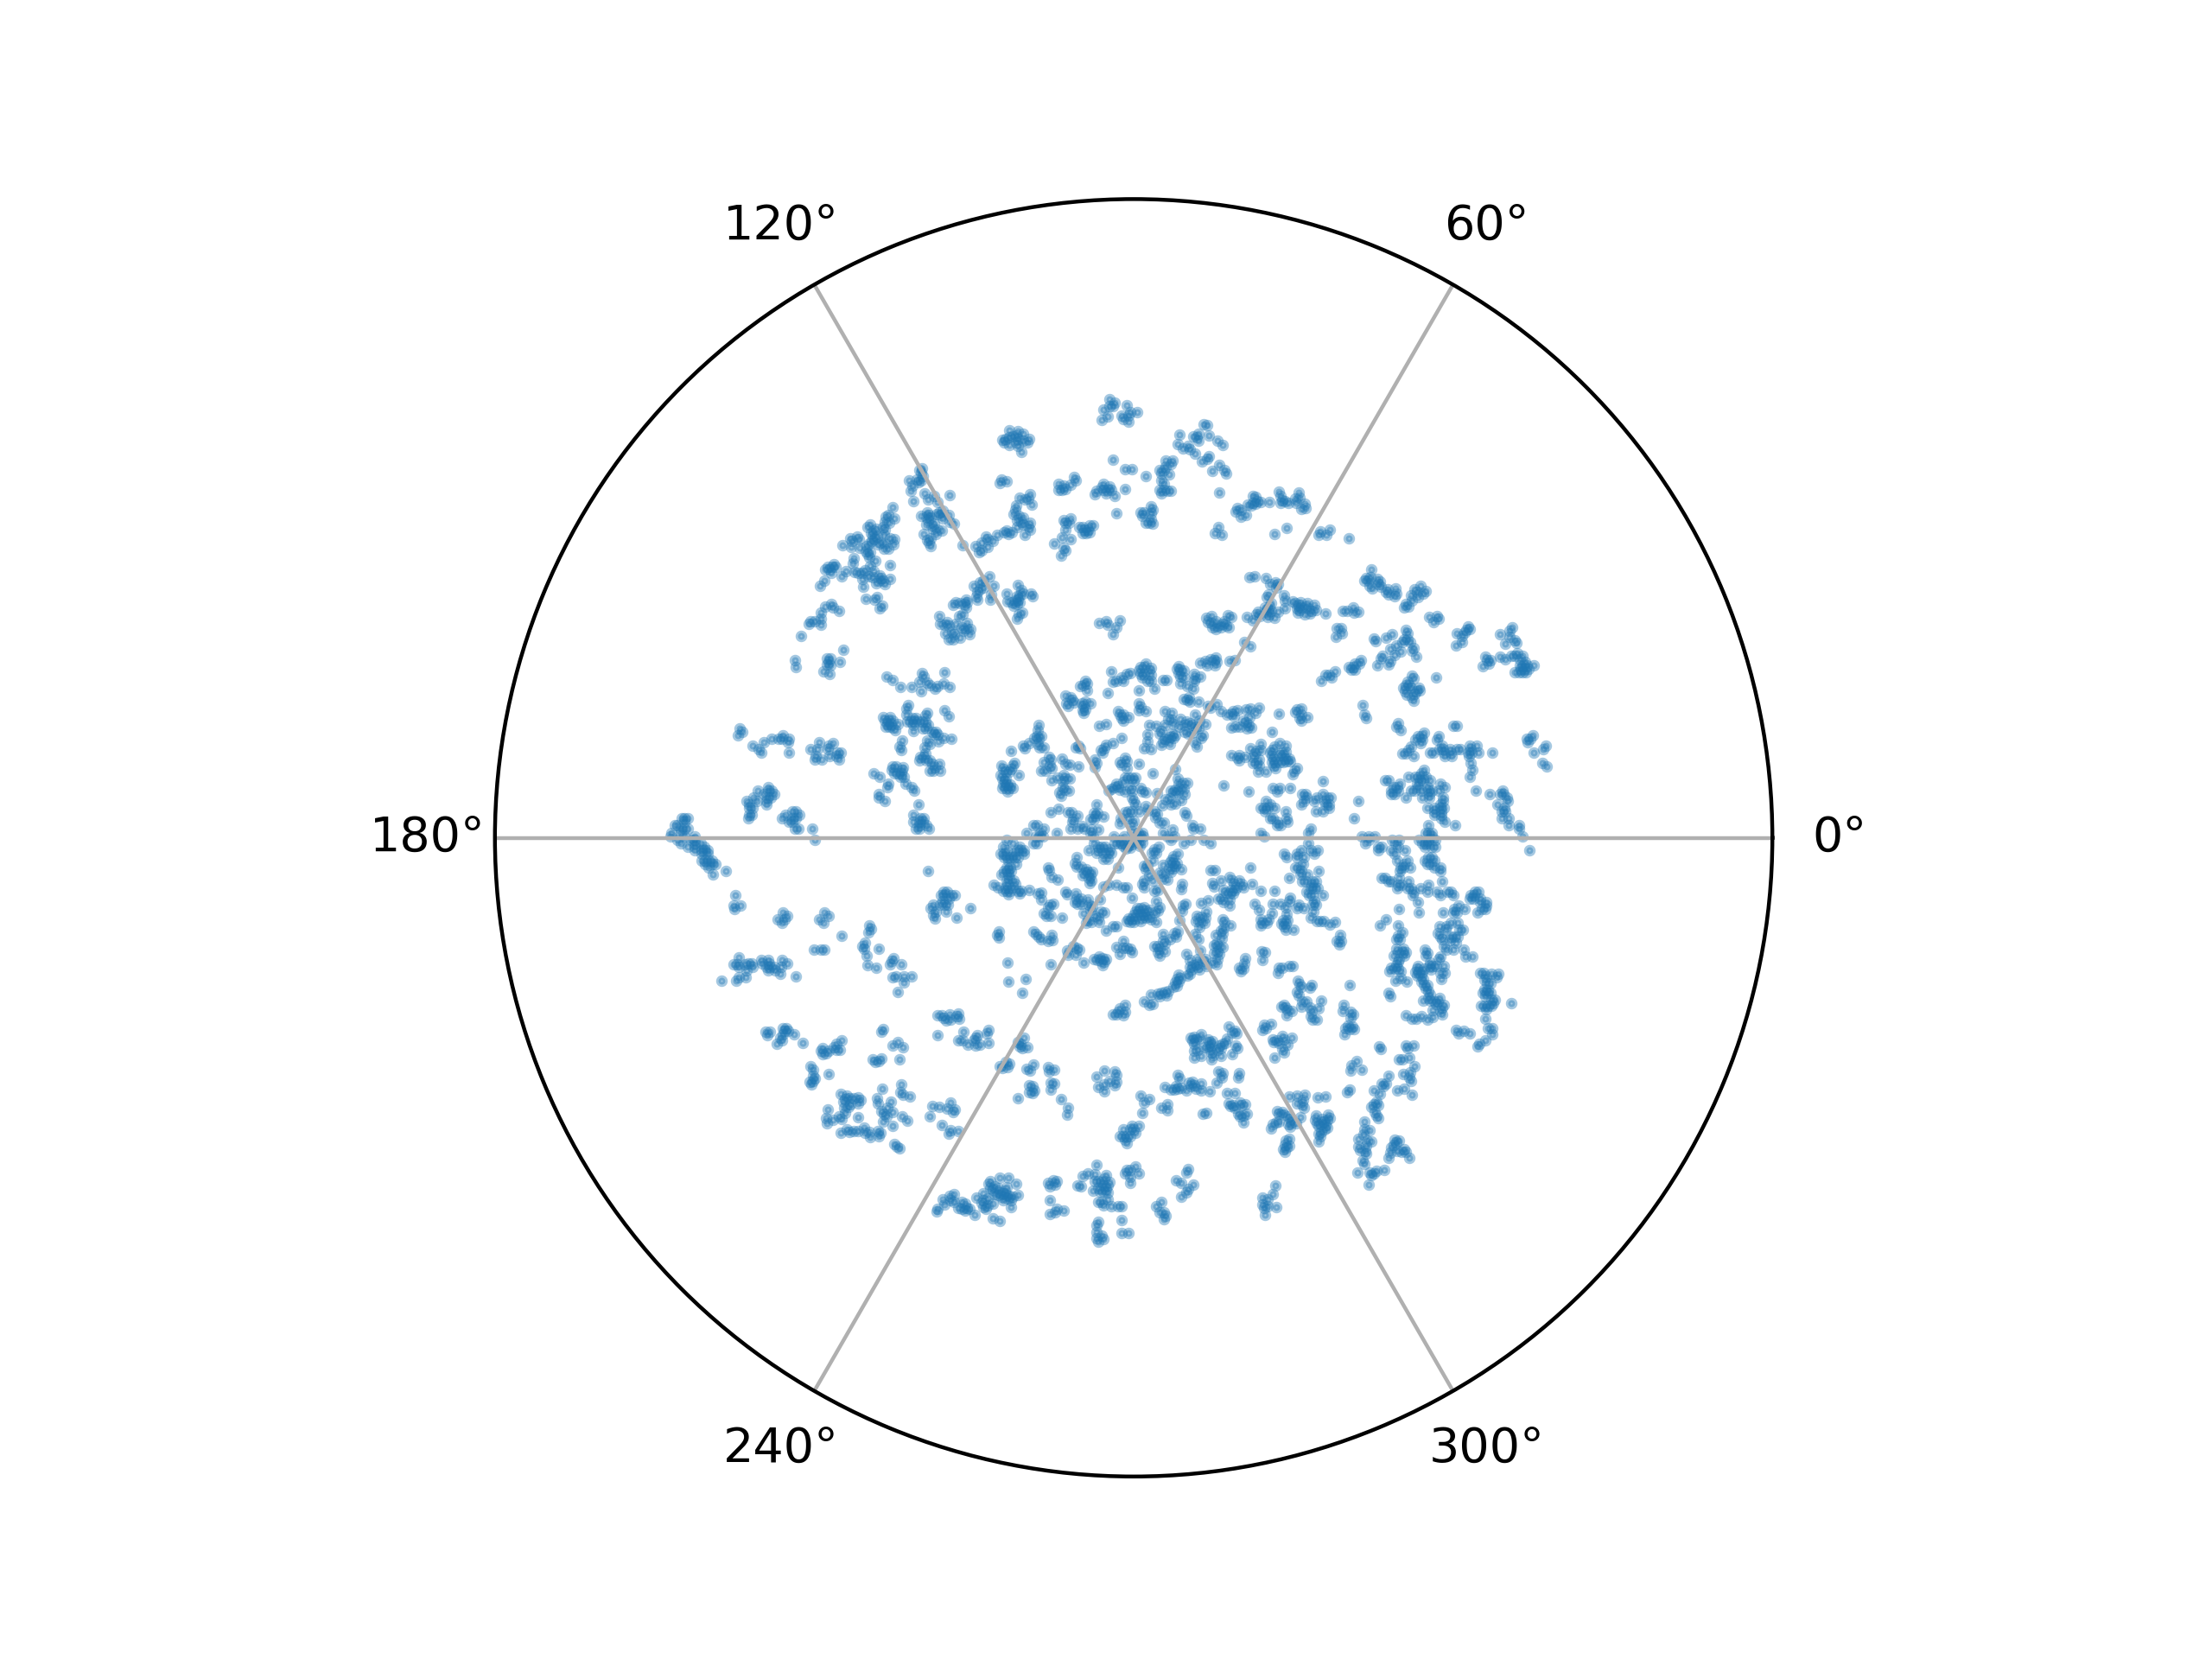
\includegraphics[width=\columnwidth]{galaxySimulationAfter.png}
            \caption{Distribution after 300 steps ($300 Myr$)}
            \label{fig:after}
        \end{subfigure}
   \caption{Simulation of galaxy formation using Yoshino and Sagawa's formalism}
   \label{fig:beforeAfter}
   \end{figure}  

\section{Conclusion}

In this essay, we have seen an introduction to the ways that Monte Carlo Methods are being used to understand the formation and evolution of galaxies. We initially introduced the concept of overdensities, that galaxies form from the gradual accretion of matter that was originally very homogeneous. We then introduce some of the characteristics of galaxies, such as their mass, fractional dimension and metallicity and then several Monte Carlo Methods that are relevant to this problem. We then discussed Henriques et al.'s use of MCMC methods for parameter estimation, Sahijpal and Kaur's stochastic model of elemental abundance and finally, we replicated Yoshino and Sagawa's simulation of the formation of spiral galaxies. Lastly, we discussed the importance of this result in verifying experimental observations of the fractal dimension.


\FloatBarrier

\onecolumngrid
\newpage

\section{References}
\bibliography{3103Essay}

\newpage

\section{Code}

The code used to create the spiral galaxy simulation from Figure \ref{fig:beforeAfter} is shown below.

\lstinputlisting[language=Python]{code/main.py}
\lstinputlisting[language=Python]{code/GalaxySimulation.py}

\end{document}



